\documentclass[10pt]{article}
\usepackage{icmlko}

\icmlmeta{IP 파운데이션 월드모델}{279}{청력}{웹툰에서는 정식화 일곱이 다 똑같다 --- 갈리는 것은 팝업에서고, 그래서 판이 못 본다}

\begin{document}

\twocolumn[
\icmlheader

\begin{abstract}
노트 278이 정식화 일곱의 ``성질표''를 만들면서 기전 셋으로 묶었다 ---
잎 하한 · 도메인별 배합 · 순수 풀링. 표현이 ``어떤 정식화는 전용 열에 눈이
멀어 있다''였다. \textbf{통제를 안 돌린 채로 그렇게 썼다.} 같은 실험을
웹툰(학습 2,106행)에 돌렸다. \textbf{일곱이 전부 쓴다} --- $+$0.5260 부터
$+$0.7354 까지고 \textbf{팝업에서 정확히 0 이던 셋(F10 · F8 · F18)도 웹툰에서는
$+$0.7354 · $+$0.5260 · $+$0.5490 이다.} F10은 최하에서 \emph{최상}으로 간다.
\textbf{눈먼 정식화 같은 것은 없었다.} 있는 것은 \textbf{청력 차이}다 ---
얼마나 작은 도메인까지 그 도메인의 전용 열을 들을 수 있나. 웹툰에서 일곱의
폭이 0.526$\sim$0.735(비 1.4배)인데 팝업에서는 0.000$\sim$0.634(비
\textbf{무한})다. \textbf{큰 도메인에서는 일곱이 사실상 같은 모형이고, 다른
모형이 되는 것은 작은 도메인에서뿐이다.} 그리고 판 $\rho$ 는 큰 도메인이
지배한다(웹툰 27.3\% · 애니 23.6\%로 둘이 절반). \textbf{그래서 판정치는
일곱을 가르는 유일한 성질을 구조적으로 못 본다} --- 못 보는 이유가 노트
274의 몫 가중 그 자체다. 노트 278이 ``상위 셋이 눈멀어 있다''고 쓴 것은
맞지만 인과가 아니었다. 맞는 문장은 이것이다 --- \textbf{판은 청력에 대해
아무 말도 안 하고, 그래서 우리는 270 노트 동안 청력을 모르고 골라 왔다.}
\end{abstract}
]

\section{통제를 안 돌렸다}

노트 278이 팝업(관측 학습 14행)에 라벨 순위를 전용 열로 주고 일곱을 쟀다.
셋이 정확히 0 이었고, 기전을 잎 하한과 도메인별 배합으로 갈랐다. 표가
깔끔했다.

\textbf{그런데 그 표에는 한 도메인밖에 없다.} ``F10은 전용 열을 못 쓴다''와
``F10은 \emph{작은} 도메인의 전용 열을 못 쓴다''는 다른 문장이고, 팝업
하나로는 안 갈린다. 노트 278의 ``남은 것''에 ``큰 도메인에서도 재기''를
적어 놓고 돌렸다.

\section{웹툰에서는 일곱이 다 쓴다}

\begin{figure*}[t]
\centering
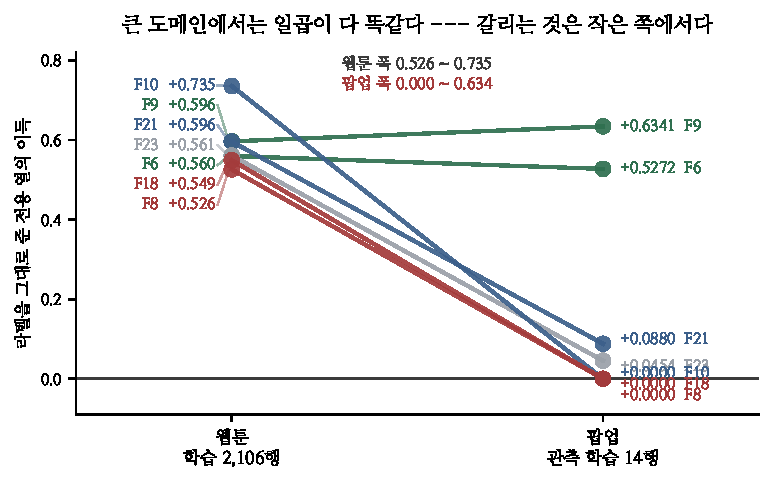
\includegraphics[width=\textwidth]{figs/hearing.pdf}
\caption{같은 실험을 두 도메인에서. 왼쪽 끝이 웹툰(학습 2,106행), 오른쪽 끝이
팝업(관측 학습 14행). 선 하나가 정식화 하나다. 색은 노트 278의 기전 묶음이다.}
\end{figure*}

\begin{center}\small
\begin{tabular}{lrrr}
\hline
정식화 & 웹툰 2,106행 & 팝업 14행 & 비 \\
\hline
F9\_ranklik & $+$0.5964 & $+$0.6341 & 1.06 \\
F6\_directpool & $+$0.5597 & $+$0.5272 & 0.94 \\
F21\_recentpick & $+$0.5957 & $+$0.0880 & 0.15 \\
F23\_rankmix & $+$0.5610 & $+$0.0454 & 0.08 \\
\textbf{F10\_pershrink} & \textbf{$+$0.7354} & \textbf{$+$0.0000} & 0.00 \\
F8\_boost & $+$0.5260 & $+$0.0000 & 0.00 \\
F18\_bagboost & $+$0.5490 & $+$0.0000 & 0.00 \\
\hline
\end{tabular}
\end{center}

\textbf{일곱이 전부 쓴다.} 그리고 \textbf{F10이 제일 잘 쓴다}($+$0.7354) ---
팝업에서 정확히 0 이던 바로 그 정식화다. 기전으로 보면 앞뒤가 맞는다:
F10은 도메인마다 ``제 이력 대 남의 이력''의 비를 따로 정하는데, 웹툰은 제
이력이 2,106행이라 배합이 제 쪽으로 쏠리고 그러면 제 전용 열이 제일 크게
일한다. \textbf{같은 기전이 팝업에서는 정반대로 작동한다} --- 14행이면 배합이
남 쪽으로 쏠리고 남에게는 그 열이 없다.

\paragraph{노트 278의 표현을 고친다} ``눈먼 정식화''는 없다. \textbf{정식화마다
들을 수 있는 도메인 크기가 다를 뿐이다.} 노트 278이 기전 셋을 옳게 짚었지만
그것을 ``어떤 것은 못 쓴다''로 적은 것이 틀렸다. 이틀 연속 같은 종류의
정정이다 --- 노트 277이 ``능형 대 나무''로 묶었다가 F10에 막혔고, 노트 278이
``눈이 멀었다''로 묶었다가 웹툰에 막혔다. \textbf{두 번 다 통제 하나가
빠져 있었다.}

\section{그래서 판이 못 본다}

수를 이렇게 놓으면 이 노트의 요점이 나온다.

\begin{center}\small
\begin{tabular}{lrr}
\hline
& 웹툰 2,106행 & 팝업 14행 \\
\hline
일곱의 최소 & $+$0.5260 & $+$0.0000 \\
일곱의 최대 & $+$0.7354 & $+$0.6341 \\
\textbf{폭} & \textbf{0.209} & \textbf{0.634} \\
최대/최소 & 1.40배 & $\infty$ \\
\hline
\end{tabular}
\end{center}

\textbf{큰 도메인에서 일곱은 사실상 같은 모형이다.} 폭 0.209는 라벨을
통째로 준 열에 대한 반응 차이니까 실제 축에서는 훨씬 작다. 일곱이 서로
\emph{다른 모형}이 되는 자리는 \textbf{작은 도메인뿐}이다.

그런데 판 $\rho$ 는 유보 표본 수로 가중한다 --- 웹툰 27.3\% · 애니 23.6\%
로 둘이 절반이고, 팝업 2.3\% · 아이돌 1.0\% 다. \textbf{판은 일곱이 서로
같은 자리에서 재고, 일곱이 갈리는 자리는 안 본다.}

이것이 노트 274의 몫 가중 이야기가 도달하는 곳이다. 노트 274는 ``작은
도메인의 개선을 판이 못 본다''였고, 여기서는 한 겹 더 나아간다 ---
\textbf{작은 도메인은 정식화들이 서로 달라지는 유일한 자리이기도 하다.}
그래서 판정치가 못 보는 것은 개선 하나가 아니라 \textbf{정식화 사이의 차이
그 자체}다.

\paragraph{그래도 눈금을 안 바꾼다} 노트 268의 규약이 그대로 산다 ---
판정 눈금을 바꾸자면 두 눈금으로 줄을 세워 보고 순위가 같으면 안 바꾼다.
그리고 이 노트가 잰 것은 \textbf{라벨을 통째로 준 진단용 열}이지 진짜
축이 아니다. 노트 277이 확인한 대로 지금 팝업에 쓸 전용 정보는 없다
(진짜 축 넷은 능형에서도 $-$0.0070).

바뀌는 것은 셋이다. \textbf{(1)} 승격 기록에 청력을 같이 적는다.
\textbf{(2)} 얇은 도메인을 실제로 쓸 결정이 서면 그때는 판 $\rho$ 가
정식화를 골라 주지 않는다는 것을 알고 시작한다. \textbf{(3)} 그리고
\textbf{2호 도메인(아이돌)이 이 문제를 바로 만난다} --- 첫 뱅크가
$n{\approx}250$ 이고, 지금 판의 아이돌은 학습 54행이다.

\paragraph{남은 것}
\begin{center}\small
\begin{tabular}{ll}
\hline
갈래 & 왜 \\
\hline
청력 곡선 & 도메인 아홉 전부 $\times$ 정식화 일곱 \\
아이돌 54행 & 벼랑 바로 위 --- 기전 셋이 거기선? \\
성질표를 루프에 & 승격 때 청력을 같이 적기 \\
배합비 직접 꺼내기 & F10의 팝업 대 웹툰 배합을 눈으로 \\
\hline
\end{tabular}
\end{center}

\paragraph{규약} \textbf{``어떤 것은 X를 못 한다''를 쓰기 전에 X를 할 수
있는 조건에서 한 번 더 잰다.} 노트 277 · 278이 이틀 연속 통제 하나가 없어
좁혀졌다. 그리고 \textbf{정식화를 견주는 실험은 큰 도메인에서 하면 아무것도
안 나온다} --- 거기서는 일곱이 같다.

\end{document}
